\chapter{Patient-Adaptable ECG Classification Framework}

\section{Introduction}

For decades, automatic ECG signal processing and analysis have been a controversial research topic. Studies carried out by scholars have proved that the development of automatic ECG analysis is conducive to the timely detection and therapeutic intervention of heart disease. However some major challenges need to be resolved before apply automatic ECG analysis as a highly reliable and fully automatic electrocardiogram processing system in clinical diagnosis. One of the most typical challenge is the inter-patient variation of ECG waveforms, which leads to inconsistent performance of ECG classification system. In this chapter, the basic framework of the proposed Patient-Adaptable ECG Classification will be discussed.

The goal of automatic ECG analysis is to determine the arrhythmia types for each signal sample. Continuous ECG signal is firstly segmented into individual segments which represent heartbeat and processed by designed algorithms. The first sections in this chapter focus on the data preparation stage, which includes four steps: signal preprocessing, delineation and segmentation, and feature extraction. Following the data preparation Section 2.2 elaborate on the framework of a two staged hierarchical classifier. The classification system is patient adaptable by capturing the normal range for each individual. More specifically, in Section 2.3, the personal dynamic normal cluster method is discussed. One feature of this method is that the cluster can dynamically adapt to patient's ECG waveform change. In many application scenarios, the physicians need to monitor long-term real-time heart activity. The dynamic adjusting system is able to address the issue of intra-patient signal variation as well

%In many application scenarios, the method of manual analysis is too complicated and time-consuming to implement. In addition, automatic electrocardiogram analysis has a very important role in monitoring long-term real-time heart activity, because manual monitoring and interpretation are not feasible under these application scenarios. It can be seen that the development of a reliable automatic heartbeat classification algorithm will be conducive to the diagnosis of arrhythmia, so this study will focus on this issue.

%The main goal of this chapter is to introduce the basic framework of automatic heartbeat classification, including ECG signal processing, characterization and classification. The rest of this chapter is organized as follows: Section 2.2 elaborated on the first step of ECG analysis, namely the preprocessing of ECG signals, including filtering and denoising; Section 2.3 immediately follows the previous section, and described the detection methods and periodic segmentation methods for the various peaks in the cardiac cycle. In particular, the multi-stroke segmentation method used in the algorithm described in this article was explained in detail; Section 2.4 introduced the steps of feature extraction and the feature quantities used in this paper based on the segmentation method used in this algorithm. The last section 2.5 is a summary of the contents of this chapter. The author reduced all the steps before the classification algorithm to a mapping and briefly outlined the structure of the classification algorithm.

\section{ECG Signal Processing}

\subsection{Preprocessing}
Biomedical signal, such as ECG signal, is often present accompanied with statistical features which change over time. Therefore, the traditional Fourier transform is not suitable for this type of non-stationary signals since it's unable to capture time-varying statistics in the signal. Wavelet decomposition solves this problem by scaling and translating mother wavelet to constitute its basis functions. Given a time series, wavelet decomposition decompose the signal into linear combinations of the aforementioned basis functions. Thus, the basis functions with large scale is wider than those with small scale and consequently correspond to low frequency component of the signal. Similarly, the coefficients of decomposition correspond to high frequency when scale is small. As such, the algorithm can extract time and frequency features through wavelet decomposition. 

Hence, in this work, wavelet analysis is applied to signals in MITDB with a sampling frequency of 360 Hz. With this sampling frequency, the decomposition coefficients and its frequency components are deduced in Fig.\ref{fig:wavelet_decomp}.

Low frequency noise or baseline wander between 0.15 to 1 Hz, cause by respiration and body movement, can be removed by deducting approximation coefficient of level 8 ($A_8$) from the signal. Since the power of ECG signal is mainly located in the frequency band from 1 to 40 Hz, some high frequency noise including electromyogram induced noise and mechanical forces acting on the electrodes can be removed by discarding the detail coefficient of level 1 ($D_1$). Daubechies wavelet of order 8 ($db8$) is selected as mother wavelet for denoising stage in this work for its optimal performance\cite{denoise}.

\subsection{Segmentation}

Among a continuous ECG signal, the characteristics of a single cardiac cycle in the signal is generally considered as a sample in most machine learning applications. Therefore, it is necessary to segment ECG signal before feature extraction. Most of the methods in literature used wavelet analysis to detect the highest peak R wave in a cardiac cycle and then detect and segment it by the amplitude-frequency characteristics of other waves. In this study, the R feature peak segmentation method used in most of the literature is adopted. In Section \ref{sec:fiducial_peaks} it was mentioned that a cardiac cycle consists of five basic characteristic peaks: P, Q, R, S, and T. Among them, the QRS complex is the most significant peak in one cycle. The energy of ECG signal in one cardiac cycle is mainly concentrated in the QRS complex. The QRS complex also contains important information that reflects the arrhythmia category\cite{2012qrs}. Accurate detection of QRS complexes is of crucial importance for subsequent analysis. The energy of the QRS complex is generally within the range of 5-25 Hz. For ECG signals with sampling frequency of 360Hz, the QRS complex information can be extracted from the detail coefficients of level 5 ($D_5$) and level 6 ($D_6$)

\begin{figure}[t]
\centering

\includegraphics[scale=.5]{Fig/scale_wavelet.png}
\caption{Frequency band of wavelet decomposition coefficient for MITDB signals}
\label{fig:wavelet_decomp}
\end{figure}


The mother wavelet $db4$ is utilized at this stage due to its morphological similarity to QRS complexes. By superimposing $D_5$ and $D_6$, the QRS complex information in the ECG signal can be characterized in a one-dimensional recombination signal ($QRS\_DET = D_5+D_6$).Other fiducial peaks (P, QRS onset, Q, S, QRS offset and T waves for each cardiac circle) are localized according to the algorithm suggested by \cite{2012qrs}. As shown in Fig.\ref{fig:QRS_d5d6}

\begin{figure}[t]
\centering
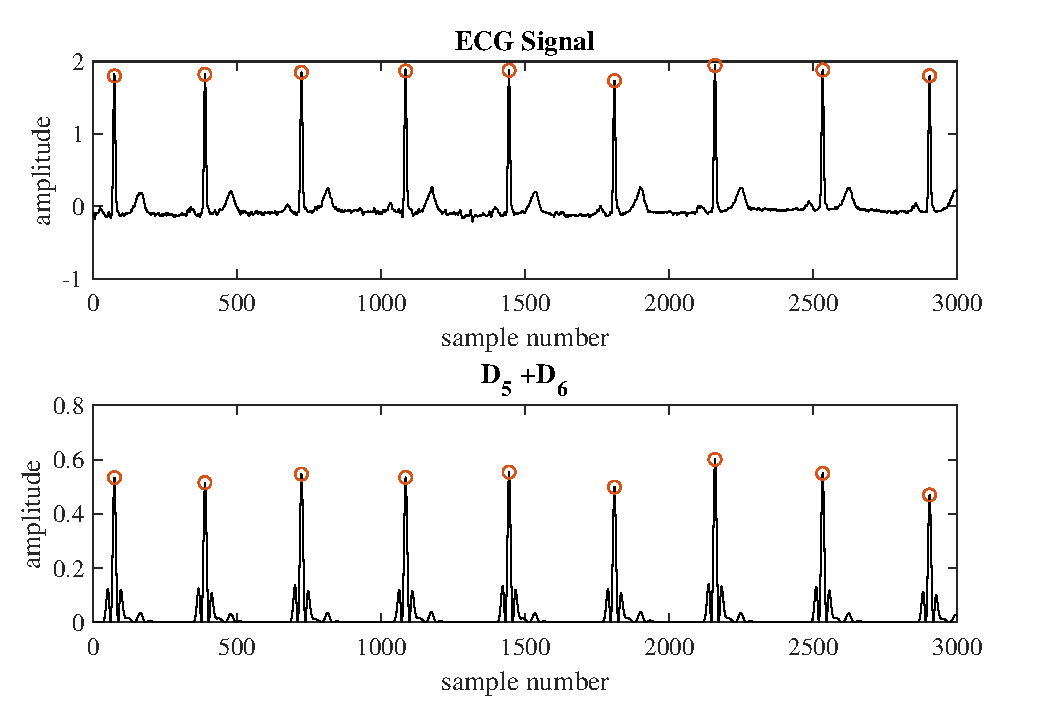
\includegraphics[scale=.7]{Fig/QRS_D5D6.pdf}
\caption{QRS detection with wavelet coefficients of level 5 and level 6}
\label{fig:QRS_d5d6}
\end{figure}


With the empirical values described in \cite{2012qrs}, we use 15\% as the detection threshold. Since the width of most of the QRS complexes does not exceed 160ms, this work used a sliding window with a width of 160ms to detect the peaks in the $QRS\_DET$. The window's step size was set to 200ms, given that the time lag between two adjacent heartbeat cycles does not exceed 200ms.  Figure.\ref{fig:window}shows the waveform of $QRS\_DET$ and the corresponding window width of 160ms. 

The false detection peaks are eliminated within a 160ms time window Fig.\ref{fig:window}


\begin{figure}[t]
\centering
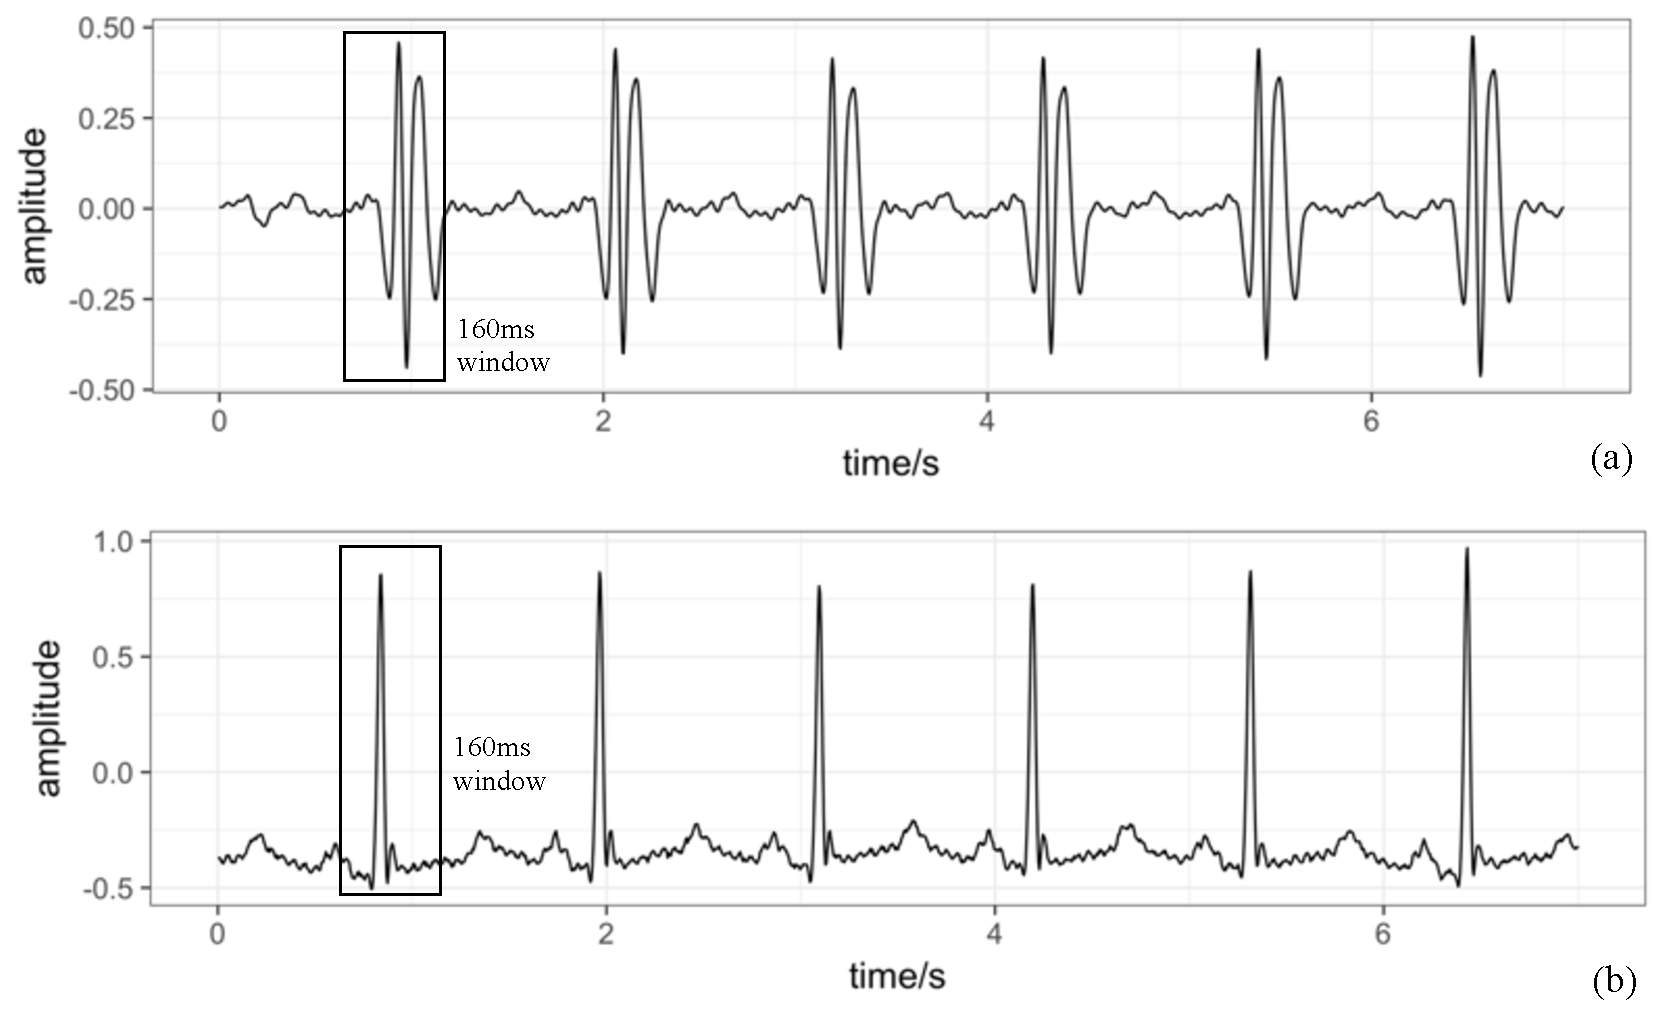
\includegraphics[scale=.5]{Fig/window.pdf}
\caption{Window for detecting R peaks within QRS complexes}
\label{fig:window}
\end{figure}


The T and P waves are outside the QRS window. By searching in a region from the start of a QRS to the end of its neighboring QRS, the P-wave is located in the highest positive peak in this region. In the same way, the position of the T wave is the position of the largest positive wave peak in the area from the end of the QRS to the next start of the next QRS. To sum up, the ECG signal in one heartbeat segment can be described by 7 feature points: P, QRS on, Q, R, S, QRS off and T. 

Finally, using the location of the R wave, a segment of the ECG signal was divided into cardiac cycles. The starting position of a cardiac cycle is defined as the position 2/3 between the R wave of the cycle and the R wave of the previous cycle. The end position is defined as 2/3 of the R wave between the cycle R and the R wave of the following cycle position. The distance (RR) between each two adjacent R waves is h. The advantage of this method is that the computational complexity is low, and the scope of application is wide and it is independent of individual patient differences. 

However the quality of ECG signals provided by most of the portable ECG measuring instruments is very unstable. Signals transmitted through wireless communication systems will exhibit various unstable waveforms. Moreover, the objective of this work is predictive modeling, thus by including statistical features capturing change between consecutive beats, the system obtains information regarding the following beats. Taking these facts into account, this work performed subsequent feature extraction and analysis combined three consecutive cardiac cycles (i.e. one representative segment). In the subsequent analysis, an segment is considered as a sample of data as shown in Fig.\ref{fig:interval}.

\begin{figure}[t]
\centering
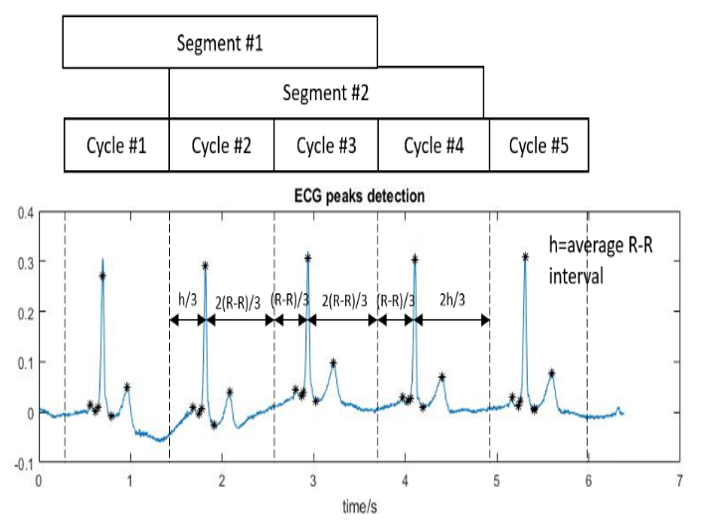
\includegraphics[scale=.8]{Fig/segment.png}
\caption{Segment samples correspond to three consecutive cardiac cycles}
\label{fig:interval}
\end{figure}


%\subsection{Dataset}

For the purpose of training and evaluating classifier, MITDB is split into test (DS2) and training (DS1) set by balancing the four classes according to \cite{autofs}. 

For each segment, a new annotation is generated by integrating all annotations of beats within the segment. Unless all beats are annotated as N within the segment, this segment will be annotated as the unique abnormality type within it. If two different abnormality types present within the same segment, this segment would be considered as transient and discarded. After segmentation and annotation generation, the total number of samples in training and test set is summarized in Table.\ref{table:ds}
\begin{table}[b]
	\centering
	\caption{Training and test datasets in MITDB.}
	\vspace{-0.05in}
	\begin{tabular}{|l||c|c|c|c|c|}
		\hline 
		& \multicolumn{4}{c}{Number of segments per AAMI class} &\\ 
		\hline 
		Evaluation Dataset& N & V & S & F &Total \\ 
		\hline 
		DS1:Training & 11721& 2356 & 862 & 256 & 15195\\ 
		\hline 
		DS2:Test & 12633 & 2053 & 550 & 121 & 15357 \\ 
		\hline 
		Total & 24354 & 4409 & 1412 & 377 & 30552 \\ 
		\hline 
	\end{tabular}
	\label{table:ds} 
	\vspace{-0.15in}
\end{table}

\section{Feature Extraction}

The feature extraction of ECG signals plays a crucial role in the diagnosis of heart disease and has a great influence on the performance of subsequent automated classification systems. De Chazal et al. discussed in detail the classification results using waveform morphological features in \cite{autofs}. As discussed in \cite{jambukia2015classification}, the combination of three types of characteristics (ie, temporal, morphology, frequency domain) can distinguish between types of arrhythmias. 

According to the related methods in literature, the different types of ECG signals mainly differ in the power level of the frequency band of 5 to 15 Hz in the segmented signal, and some other morphological features (such as the duration between the Q wave and the T wave, P The distance to the R wave, etc.) also shows a correlation with the signal class. Based on the sample segmentation method used in this paper, the feature extraction stage divided the three major types of features into periodic-based features (SET 1) and segment-based features (SET 2). Here, SET1 includes the average and standard deviation of the corresponding features of the three cardiac cycles within a segment, and SET2 contains the overall characteristics of the time signal within the segment, so it is calculated once in segment intervals. 22 feature quantities are extracted for each segment, which is then normalized to obtain a feature of zero-mean unit variance, and a 22×1 vector is used to represent the k-th segment. Summarized details are described in Table.\ref{table:features}. The mean$(R_{i+1}-R_i)$ refers to the mean of the time lag between two adjacent R waves, while $(R_i-R_{avg})$ is the length of each cardiac cycle and the average cardiac cycle duration of the patient. 

\begin{table}[t]
	\caption{Features extracted from ECG signal}
	\label{table:features}
	\centering
	%\begin{flushleft}
	\begin{tabular}{|m{6em} || @{}m{7.4em} ||@{} m{7.7em}|}
		\hline 
		Feature Type & SET1 & SET2 \\ 
		\hline 
		Temporal Features & QRS duration, ~~~~
		QT duration, ~~~~~~~
		PR duration & mean$(R_{i+1}-R_i)$, mean$(R_i-R_{avg})$  \\ 
		\hline 
		Morphological Features & max positive peak to second peak ratio & signal average energy, max positive peak, max
		negative
		peak, peak to
		energy ratio \\ 
		\hline 
		Frequency Domain Features & signal power level at 7.5Hz, 10Hz, 12.5Hz, 15Hz &  \\ 
		\hline 
	\end{tabular} 
	%\end{flushleft}
\end{table}

From Table.\ref{table:features}, it is explicit that these 22 feature are not completely independent of each other. Therefore, in this work, Principal Component Analysis (PCA) is used to reduce the dimensions of features. Finally, 8 feature quantities were obtained after dimension reduction.


\section{Classification Framework}

In this section, a system is designed to address the classification and prediction tasks based on the processed ECG data. Based on our previous study and similar works which aimed to solve patient-specific classification problem, a two-staged structured which contains a global classifier and personalized classifier is retained as outline in this paper\cite{chen2018predictive,Hu_et_al,deChazal2006,llamedo2012automatic}. Moreover, the proposed algorithm incorporates a novel deviation quantification module depicted in details in the following section. 

The framework of system is summarized by the flowchart in Figure \ref{fig:flow}. A pre-trained Global Classifier serves as preliminary classifier, it facilitates the following analysis in the system for it identifies samples with severe morbidity. Depending on applications, different conventional classification algorithms with low complexity can be considered as Global Classifier. Any abnormal labels generated by Global Classifier are considered as Red Alarms and do not require further processing.

\begin{figure}[ht]
	\centering
	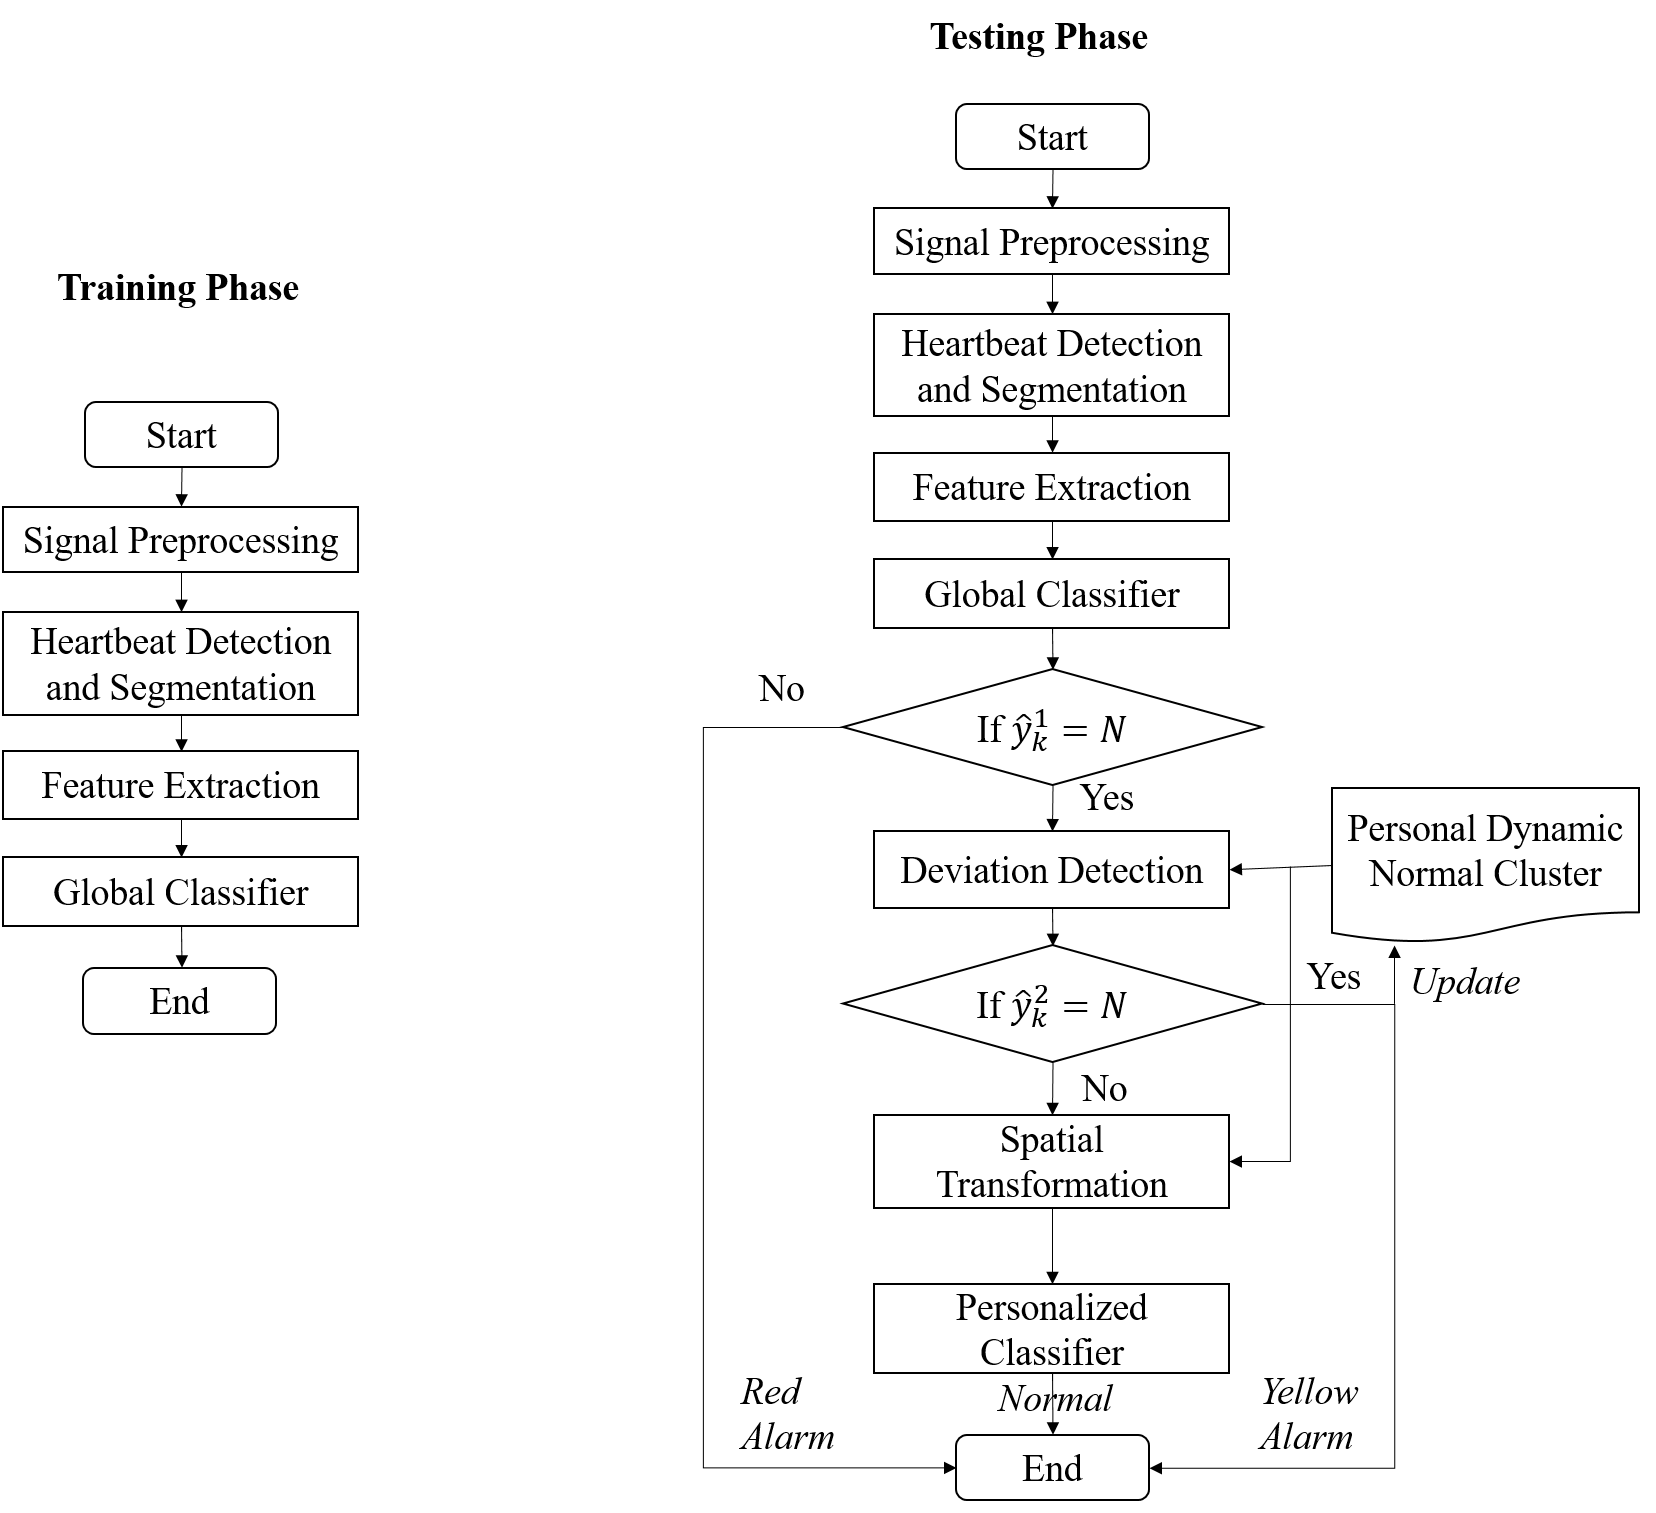
\includegraphics[scale=.5]{Fig/flow2.png}
	\caption{The general flowchart of proposed framework}
	\label{fig:flow}
\end{figure}

However, as the objective of this study is to identify latent status between normality and abnormalities, the design focus on processing samples classified as N while deviating towards abnormal classes. For this purpose, a simple structured classifier is insufficient since sample numbers of N and other morbid classes are unbalanced in training set DS1 as shown in Table.\ref{table:ds}, which results in missed abnormalities. Thus a deviation detection module is added after the Global Classifier to specifically identify latent status using patient-specific normal cluster. In order to extract patient-specific information and adapt the classifier accordingly, the first 20\% of total Normal samples of each patient are selected as initialization of Personal Dynamic Normal Cluster $\mathcal{N}_0^k$. The binary classification of N versus non-N which includes all abnormal classes is completed by first calculating the following distance metrics:

\begin{align}
\label{eq:matrices}
R_i^{\max}=\underset{\mathbf{x}_j\in\mathcal{N}_i^k,\mathbf{x}_k\in\mathcal{N}_i^k}{\max}\{\sqrt{(\mathbf{x}_j-\mathbf{x}_k)^2}\},
\\
D_\mathcal{X}(\mathbf{x}_k(i))=\underset{\mathbf{x} \in\mathcal{X}}{\text{median}}\{\sqrt{(\mathbf{x}_k(i)-\mathbf{x})^2}\},
\\
D_\mathcal{N}^{\max}(\mathbf{x}_k(i))=\underset{\mathbf{x} \in\mathcal{N}_i^k}{\text{max}}\{\sqrt{(\mathbf{x}_k(i)-\mathbf{x})^2}\},
%D_V(x^t)=\underset{x_V\in\Omega_V}{\text{median}}\{\sqrt{(x^t-x_V)^2}\}\\
%D_S(x^t)=\underset{x_S\in\Omega_S}{\text{median}}\{\sqrt{(x^t-x_S)^2}\}\\
%D_F(x^t)=\underset{x_N\in\Omega_F}{\text{median}}\{\sqrt{(x^t-x_F)^2}\}\\
%D_{max}(x^t)=\underset{x_N\in\Omega_N^t}{\max}\{\sqrt{(x^t-x_N)^2}\}
\end{align}

The following conditions are thus examined to verify if deviation of a sample is within the range defined by $\alpha$. Considering the fact that some rare abnormalities are unlikely to be observed within the limit initialization time range, abnormal clusters: ${\mathcal{S},\mathcal{V},\mathcal{F}}$ ,which are composed of abnormal beats in DS1, are deployed as training data together with Personal Dynamic Normal Cluster $\mathcal{N}_i^k$ in the following steps.

\begin{align}\label{eq:condition1}
\begin{cases}
D_\mathcal{N}^{\max}(\mathbf{x}_k(i))  \leq\alpha R_i^{\max},\\
D_\mathcal{N}(\mathbf{x}_k(i)) < D_\mathcal{X}(\mathbf{x}_k(i)) &\text{for~} \mathcal{X}\in\{\mathcal{S},\mathcal{V},\mathcal{F}\}   %(D_N(x^t),D_V(x^t),D_S(x^t),D_F(x^t))=D_N(x^t)
\end{cases}
\end{align}

If a sample is confirmed as N in this module, it will be used to update the $\mathcal{N}_i^k$. Otherwise the system assumes that the sample have demonstrated deviation towards abnormal clusters and will pass it to the subsequent Personal Classifier with controlled nonlinear transformation. Using transformation with optimized parameters, Personal Classifier is able to discern the deviation to different morbid types regardless of the cluster topology within the original feature space. Details of the module will be presented in the next Section.

Overall, if given a sample $x_k$ at time $k$, the proposed framework maps it to label $\hat{y}_k \in \{N,Y_V,Y_S,Y_F,R_V,R_S,R_F\}$, where $N$ stands for normal, $Y_V$ stands for ventricular yellow alarm, $R_V$ stands for ventricular red alarm.

\begin{figure}[t]
\centering
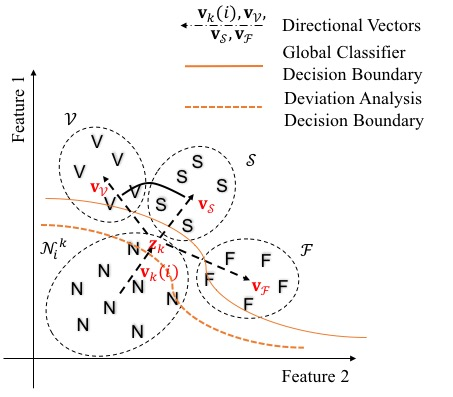
\includegraphics[scale=.7]{Fig/topology.jpg}
\caption{The deviation analysis boundary restrict on latent status between normal and abnormal samples compared with the Global Classifier boundary}
\label{fig:topo_deviation}
\end{figure}


\section{Personal Classifier}

As the proposed system aims at predicting subsequent abnormalities by analyzing the deviation of sample signal, it's vital to quantify the deviations using topological characteristics of training data. For most of the ECG applications analysis is conducted within high-dimensional feature space, we therefore select Cosine Distance(defined in Eq.\ref{eq:cosine}) to quantify deviation.

\begin{align}
\label{eq:cosine}
d(\mathbf{v},\mathbf{w})= 1 - \frac{\mathbf{v}^T\mathbf{w}}{|\mathbf{v}||\mathbf{w}|}=1 - \frac{\mathbf{v}^T\mathbf{w}}{\sqrt{(\mathbf{v}^T\mathbf{v})(\mathbf{w}^T\mathbf{w})}}
\end{align}

Consequently, relative deviations of sample from normal cluster(N) to other abnormal clusters (V, S, F) are defined by cosine distance between the vector $\mathbf{v}_k(i)$ (defined in Eq.\ref{eq:v_k}) to three vectors $\mathbf{v}_{\mathcal{X}}(i)=\mathbf{c}_{\mathcal{X}}-\mathbf{x}_k(i)$ where $\mathcal{X} \in \{ \mathcal{S}, \mathcal{V}, \mathcal{F}\}$. In this case, smaller cosine distance represents higher alignments between normal cluster centroid $\mathbf{v}_k(i)$, current sample $\mathbf{x}_k(i)$ and the abnormal centroid $\mathbf{c}_{\mathcal{X}}$.


\begin{align}
\label{eq:v_k}
%\mathbf{v}_k=\mathbf{x}_k-\mathbf{c}_N^k = \mathbf{x}_k- \frac{\sum_{j=1}^{k-1} \mathbf{x}_j I(\hat{y}_j=N)}{\sum_{j=1}^{k-1}  I(\hat{y}_j=N)}, 
\mathbf{v}_k(i)=\mathbf{x}_k(i)-\mathbf{c}_N^k(i) = \mathbf{x}_k(i)- {\sum_{\mathbf{x} \in \mathcal{N}_i^k} \mathbf{x}}/{|\mathcal{N}_i^k|}, 
\end{align}

Therefore the classification results of Personal Classifier $\hat{y}^2_k(i)$ is defined as follows:

\begin{align}
\label{eq:personal_discrim}
\hat{y}^2_k(i) = \underset{\mathcal{X} \in \{ \mathcal{S}, \mathcal{V}, \mathcal{F} \}}{\text{argmin}}\{ d(\mathbf{v}_k(i),\mathbf{v}_{\mathcal{X}}(i)) \} 
\end{align}

The measurement accuracy of cosine distance varies according to topology of clusters in feature space. Whereas the topology in feature space relies on feature extraction and feature selection. For example, as shown in Fig.\ref{fig:topo1}, in the original feature space overlaps and alignment of abnormal clusters may lead to inaccurate results of deviation quantification. In order to avoid the ambiguity, a topology where abnormal clusters encircle normal cluster is required.

\begin{figure}[thpb]
\centering
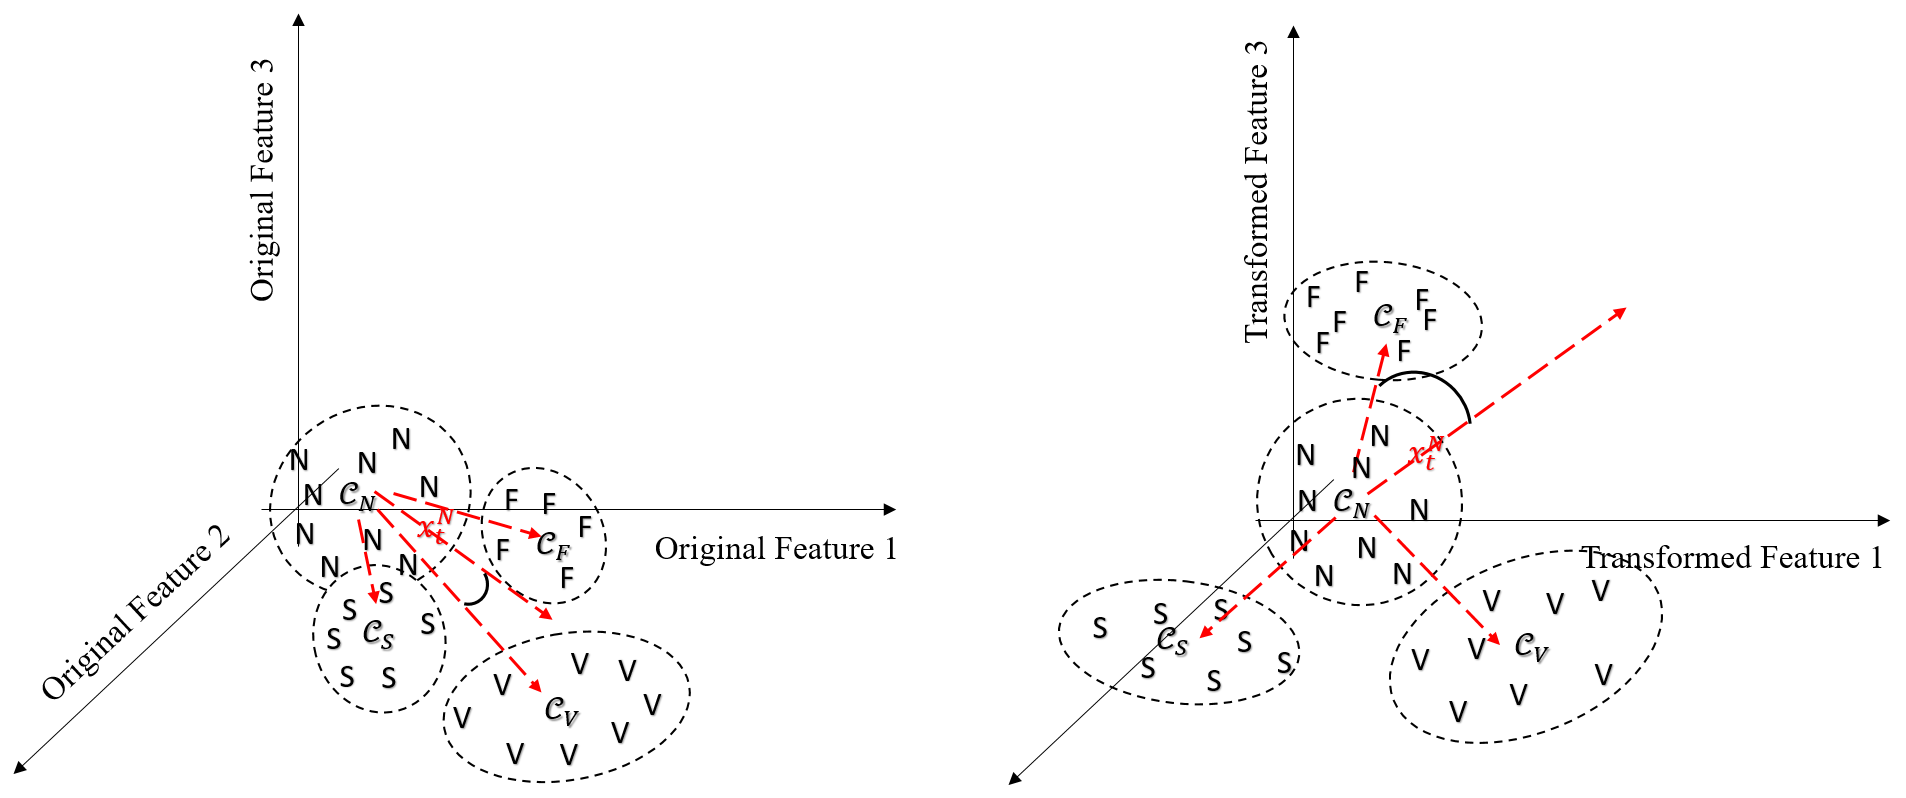
\includegraphics[scale=.5]{Fig/topo1.png}
\caption{Left: illustration of cluster topology in original feature space; Right: illustration of cluster topology in feature space transformed with simple mapping function}
\label{fig:topo1}
\end{figure}

For this purpose, two different spatial transformation methods are proposed in the next two chapters.